\newpage
\subsection{Caso d'uso UC1: Main pre-autenticazione }
\label{UC1}
\begin{figure}[ht]
	\centering
	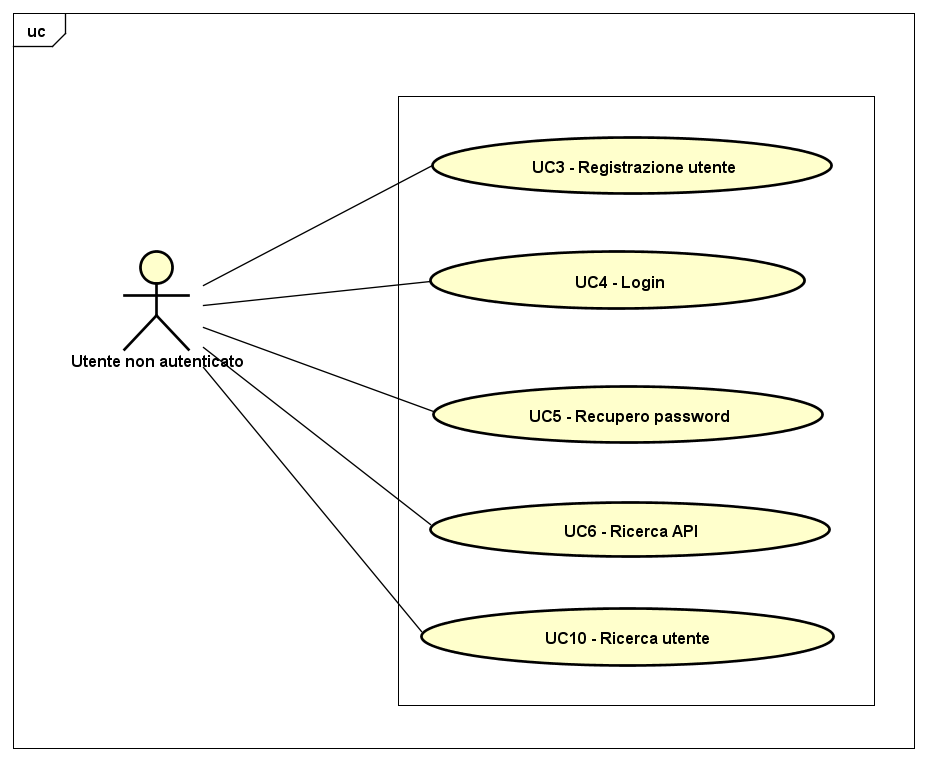
\includegraphics[scale=0.45]{UML/UC1.png}
	\caption{UC1: Main pre-autenticazione}
\end{figure}

\renewcommand*{\arraystretch}{1.6}
\begin{longtable}{ l | p{11cm}}
	\hline
	\rowcolor{Gray}
	 \multicolumn{2}{c}{UC1 - Main pre-autenticazione} \\
	 \hline
	\textbf{Attori} & Utente non autenticato  \\
	\textbf{Descrizione} & L'attore, tramite la schermata principale dell'applicazione, può accedere e sfruttare le funzionalità a lui disponibili: la registrazione, il login, il recupero password, la ricerca API  \\
	\textbf{Pre-Condizioni} & L'attore ha avviato l'applicazione web e non si è ancora autenticato \\
	\textbf{Post-Condizioni} & L'applicazione ha eseguito le richieste dell'attore\\
	\textbf{Scenario Principale} & \begin{enumerate*}[label=(\arabic*.),itemjoin={\newline}]
		\item L'attore può registrarsi all'applicazione (UC3)
		\item L'attore può effettuare il login all'applicazione (UC4)
		\item L'attore può recuperare la propria password (UC5)
		\item L'attore può effettuare una ricerca sulle API presenti nell'applicazione (UC6)
		\item L'attore può effettuare una ricerca sugli utenti registrati all'applicazione (UC10)
	\end{enumerate*}\\
\end{longtable}